\chapter{Implementation Details}
This is where you explain what you have implemented and how you have implemented it. Place here all the details that you consider important, organize the chapter in sections and subsections to explain the development and your workflow.\\Given the self-explicative title of the chapter, readers usually skip it. This is ok, because this entire chapter is simply meant to describe the details of your work so that people that are very interested (such as people who have to evaluate your work or people who have to build something more complex starting from what you did) can fully understand what you developed or implemented.\\Don't worry about placing too many details in this chapter, the only essential thing is that you keep everything tidy, without mixing too much information (so make use of sections, subsections, lists, etc.). As usual, pictures are helpful.

\section {Device side}

The operations that the device must be able to perform are two:
\begin{itemize}
	\item Read the PUFs from the RAM and store them in the SRAM, to be done the moment the device is powered on.
	\item Given a challenge,  compare the PUF found in the DB of PUFs and the one found in the SRAM.
\end{itemize}

The implementation of both functionalities is based on the provided code and changes to it have been made to fit our purpose.

\subsection{Generation of PUFs}

To make the retrieval of the PUFs possible two files had to be changed
\begin{enumerate}
	\item $USBStick > Startup > startup\_stm32f429nihx.s$
	\item $USBStick > Src > Device > se3\_dispatcher\_core.c$
\end{enumerate}

The .s file is the one in which the reset handler can be found and it will be executed before the main. Since the the content of the RAM will be overwritten the PUFs must be copied as soon as possible. For this reason this operation has been done before any memory initialization.

Using the reference manual for the MCU (STM32f429) we know the memory mapping of both the SRAM(0x020000000 -  0x02002FFFF) and flash memory(0x08000000 - 0x081FFFFF). Starting from that we scanned the SRAM and loaded the content to a part of the flash memory that will not compromise sensible data.

Since the the flash memory needs control registers to be set to guaranty access we called the HAL functions in the assembly code. More precisely the functions to unlock and program/write in memory. The code written to perform this operation is provided in figure \ref{fig:code_assembly}

\begin{figure}[h!]
	\vspace{0.5cm}
	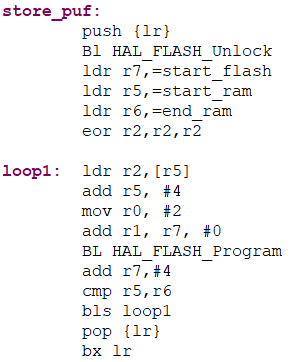
\includegraphics[width = 0.3\textwidth]{images/code_assembly.png}
	\caption{Assembly code to store PUFs into the flash memory. }
	\label{fig:code_assembly}
\end{figure}

At the end of the execution of this code we expect a number of PUFs to be stored in the flash memory which will be accessible once we enter the main and enter the execution loop where we can call our functions and access the content of the SRAM

Once we have the PUFs in memory we need to able to access them. This is done through the execution of two functions $puf\_retreive()$ and $puf\_challenge()$. These two functions are the ones that will be called when the appropriate command will be sent from the host towards the device. These two functions can be found in the $se3\_dispatcher\_core.c$ file.

To make the command call possible it is necessary to define these commands in the $se3_dispatcher_core.h$ which must reflect the number associated also to the host side for the same command.

\subsubsection{puf\_retreive()}

This function is on the board side and as such it has to be called from the host side by sending, besides the parameters, the correct command code to call it. It can communicate with the host though the received and sent data and also the size of that data. The size of the received and sent data has been used as a correctness check. As for the data itself, since the host library works on bytes, also on the board side we worked with bytes. This means that the access to the SRAM is done bytewise.

This function will start from a predefined position in memory and will read e predefined number of addresses accessing the PUFs stored on startup. As a return parameter to the Host it will pass the vector of all the PUFs read. Then the Host is responsible to manage them.


\subsubsection{puf\_challenge()}

This function is called and defined in the same way as the puf\_retreive function with the difference being the actual operations performed. In fact now the Host must also provide the challenge and the challenge response so that we can read the SRAM of the board access the memory at the location indicated by the challenge and read the content expecting it to be the same as the one passed to it. In the function the comparison will be made and a found not found response will be sent back to the host.

In this case the operation is simply a read from memory but particular attention was given to the way data is sent since we are again working with bytes and a reconstruction on 32 bits will be necessary.


\section {Host side} 
\label{section:impl_host}